\section{分割算法与验证选参}
\subsection{颜色阈值与区域处理}

分割从原图的颜色开始。输入图像保持原始尺寸，以 BGR 顺序读取为 8 位整数，再通过 OpenCV 的颜色转换得到 Y、Cr、Cb。采用从 98 张训练图中提取的 6,387,552 个皮肤与鼻子像素作为颜色统计依据，参数如表~\ref{tab:skinparams} 所示。

\begin{table}[H]
\centering
\small
\caption{检测器使用的训练统计参数}\label{tab:skinparams}
\begin{tabular}{lrr}
\toprule
通道 & 均值 & 标准差 \\
\midrule
Cr & 151.14949561 & 9.37448409 \\
Cb & 109.11018055 & 9.48356505 \\
\bottomrule
\end{tabular}
\end{table}

对每个像素，同时满足式~\eqref{eq:colorbox} 时记为候选前景。系数 $k$ 控制颜色范围，范围扩大后可以保留更多脸部像素，同时也会纳入更多相近颜色的区域。
\begin{equation}
M(x,y)=\begin{cases}
1, & |Cr(x,y)-\mu_{Cr}|\leq k\sigma_{Cr}\ \text{且}\ |Cb(x,y)-\mu_{Cb}|\leq k\sigma_{Cb},\\
0, & \text{其他情况}.
\end{cases}
\label{eq:colorbox}
\end{equation}
其中，$\sigma$ 表示标准差。实现中先将通道值转为浮点数再作差，保留阈值边界，不对每张图像重新估计颜色参数。读图、颜色转换和预处理方式与训练统计保持一致。

颜色候选还需要处理空间结构。脸部真值包括眼睛、眉毛、口腔与嘴唇，这些位置未必满足肤色范围，容易在二值掩膜中形成空洞。填孔用于补回被外部轮廓包围的内部区域。图像中与脸部分离的类肤色背景则可以通过连通域筛选排除。

最终方案先按照 8 连通关系保留面积最大的前景块，再填充与图像外部背景不保持 4 连通的内部空洞。该处理适合图像中存在一个主要脸部区域的情况，处理对象始终是预测掩膜。

\subsection{验证集参数比较}

数据沿用训练 98 张、验证 32 张、测试 32 张的固定划分。验证时比较 9 个系数，取值从 1 到 3，步长为 0.25，并组合无处理、填孔、最大连通域后填孔、闭运算后最大连通域与填孔四种流程，共 36 组。闭运算使用 $5\times5$ 椭圆核，所有图像共用一套全局参数。

选参使用验证集的全局 F1，即先累加各图的混淆计数，再计算 F1。相同分数优先选择较简单的处理，再选择较小的 $k$。图~\ref{fig:valcurve} 展示了参数变化。

\begin{figure}[H]
\centering
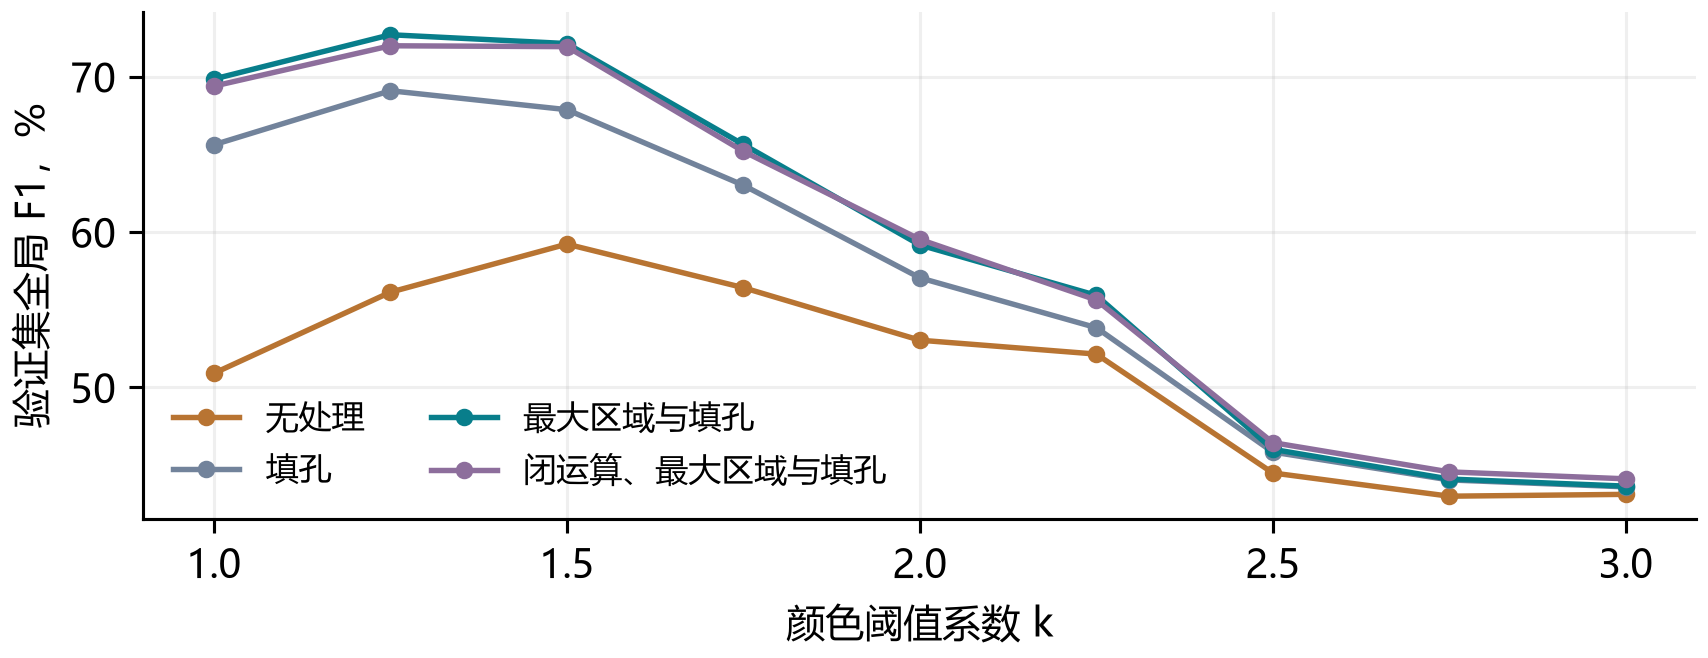
\includegraphics[width=0.96\textwidth]{validation_curve.png}
\caption{四种处理方式在验证集上的参数曲线}
\label{fig:valcurve}
\end{figure}

\begin{table}[H]
\centering
\small
\caption{固定基线与最终方案的验证结果，单位为百分比}\label{tab:validation}
\begin{tabular}{lrrrrr}
\toprule
方案 & $k$ & Precision & Recall & F1 & IoU \\
\midrule
纯阈值基线 & 1.50 & 49.44 & 73.84 & 59.22 & 42.07 \\
最大区域与填孔 & 1.25 & 64.86 & 82.70 & 72.70 & 57.11 \\
\bottomrule
\end{tabular}
\end{table}

最终选择 $k=1.25$ 的最大连通域与填孔组合，验证 F1 比纯阈值基线提高 13.48 个百分点，IoU 提高 15.04 个百分点。最终 TP、FP、TN、FN 分别为 1,842,674、998,367、5,162,119、385,448。其逐图 F1 平均为 0.706746，与按像素累计得到的全局 F1 分开记录。

为进一步看清后处理的作用，将 $k$ 固定为 1.25，比较四种流程，如表~\ref{tab:postvalidation} 所示。

\begin{table}[H]
\centering
\small
\caption{相同颜色阈值下的验证集后处理比较，单位为百分比}\label{tab:postvalidation}
\begin{tabular}{lrrrr}
\toprule
后处理 & Precision & Recall & F1 & IoU \\
\midrule
无处理 & 52.43 & 60.39 & 56.13 & 39.01 \\
填孔 & 58.34 & 84.71 & 69.10 & 52.78 \\
最大区域与填孔 & 64.86 & 82.70 & 72.70 & 57.11 \\
闭运算、最大区域与填孔 & 63.39 & 83.30 & 71.99 & 56.24 \\
\bottomrule
\end{tabular}
\end{table}

填孔后 F1 有明显提高，再加入最大区域筛选得到最高值。额外闭运算的结果略低，因此最终流程保留最大区域与填孔。颜色阈值放宽后，召回率持续上升，但误检也随之增加，最终选择体现了两者的取舍。

\begin{samepage}
\subsection{验证案例与方案固定}

按最终验证 F1 选择最差的两张图和最好的一张图，结果如表~\ref{tab:valcases} 所示。

\begin{table}[H]
\centering
\small
\caption{验证集代表样例}\label{tab:valcases}
\begin{tabular}{lrp{9.4cm}}
\toprule
样例编号 & F1 & 预测现象 \\
\midrule
00733 & 0.086946 & 类肤色背景误检，脸部主体漏检。 \\
00562 & 0.129510 & 脸部主体缺失，填孔恢复有限。 \\
00731 & 0.958894 & 脸部主体覆盖较完整，轮廓外仍有少量误检。 \\
\bottomrule
\end{tabular}
\end{table}

验证时已观察到颜色候选不足和最大区域错选。保存预测后重新读取评价，计数和主要指标与搜索时一致，随后固定两套配置进入独立测试。

\end{samepage}
